\documentclass[tikz,border=10pt]{standalone}
\begin{document}
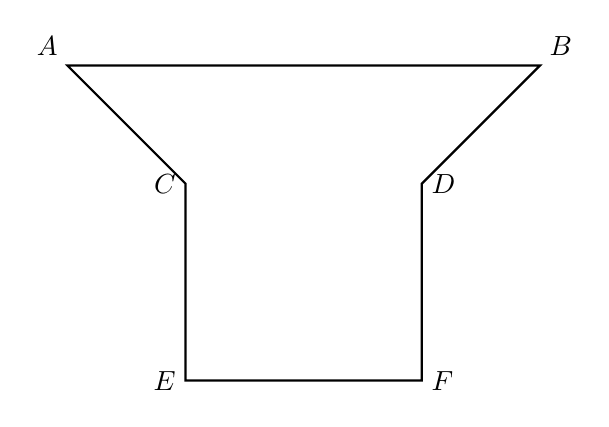
\begin{tikzpicture}
  \coordinate (A) at (0,4);
  \coordinate (B) at (6,4);
  \coordinate (C) at (1.5,2.5);
  \coordinate (D) at (4.5,2.5);
  \coordinate (E) at (1.5,0);
  \coordinate (F) at (4.5,0);

  \draw[thick] (A) -- (B) -- (D) -- (F) -- (E) -- (C) -- cycle;

  \node[above left] at (A) {$A$};
  \node[above right] at (B) {$B$};
  \node[left] at (C) {$C$};
  \node[right] at (D) {$D$};
  \node[left] at (E) {$E$};
  \node[right] at (F) {$F$};
\end{tikzpicture}
\end{document}
